\documentclass[12pt]{article} % 12pt 为字号大小 UTF8
\usepackage{amssymb,amsfonts,amsmath,amsthm}
%\usepackage{fontspec,xltxtra,xunicode}
%\usepackage{times}

%----------
% 定义中文环境
%----------

\usepackage{xeCJK}

% \setCJKmainfont[BoldFont={SimHei},ItalicFont={KaiTi}]{SimSun}
% \setCJKsansfont{SimHei}
% \setCJKfamilyfont{zhsong}{SimSun}
% \setCJKfamilyfont{zhhei}{SimHei}

% \newcommand*{\songti}{\CJKfamily{zhsong}} % 宋体
% \newcommand*{\heiti}{\CJKfamily{zhhei}}   % 黑体


%----------
% 版面设置
%----------
% %首段缩进
% \usepackage{indentfirst}
% \setlength{\parindent}{2.1em}
% 设置段落不缩进
\setlength{\parindent}{0pt}

%行距
\renewcommand{\baselinestretch}{1.2} % 1.4倍行距

%页边距
\usepackage[a4paper]{geometry}
\geometry{verbose,
  tmargin=3cm,% 上边距
  bmargin=3cm,% 下边距
  lmargin=3cm,% 左边距
  rmargin=3cm % 右边距
}


%----------
% 其他宏包
%----------
%图形相关
\usepackage[x11names]{xcolor} % must before tikz, x11names defines RoyalBlue3
\usepackage{graphicx}
\usepackage{pstricks,pst-plot,pst-eps}
\usepackage{subfig}
\def\pgfsysdriver{pgfsys-dvipdfmx.def} % put before tikz
\usepackage{tikz}

%原文照排
\usepackage{verbatim}
\usepackage{float}

%网址
\usepackage{url}

%文本格式
\usepackage{ulem} % 用法:\uline{}下划线,\uwave{}波浪线,\sout{}删除线
\usepackage{pifont} % 用法:\ding{数字}代表数字被圈起来
\usepackage{enumitem} % 使用enumitem宏包自定义列表样式
\usepackage{hyperref} % 不仅可以帮助你插入链接,还能让这些链接在生成的PDF文档中是可点击的,提高文档的互动性,用法:\url{http://www.example.com}


%----------
% 习题与解答环境
%----------
%习题环境
\newtheoremstyle{problemstyle} % 定义一个名为 problemstyle 的新风格
  {3pt} % 上部空白量
  {3pt} % 下部空白量
  {} % 正文字体
  {} % 缩进量
  {\bfseries} % 标题字体
  {} % 标题后的标点
  {\newline} % 标题后的空白
  {\underline{\thmname{#1}\thmnumber{ #2}}\thmnote{ (#3)}} % 定理头部格式

\theoremstyle{problemstyle} % 使用 problemstyle 风格
\newtheorem{problem}{题目} % 定义题目环境

%解答环境
\newenvironment{solution}
  {%
    \renewcommand\qedsymbol{$\blacksquare$}%
    \proof[\textit{解答}]\mbox{}\vspace{-4ex}\\%
  }
  {\endproof}
%----------
% 我的自定义
%----------

\newcommand{\horrule}[1]{\rule[0.5ex]{\linewidth}{#1}} 	% Horizontal rule

\renewcommand{\refname}{参考文献}
\renewcommand{\abstractname}{\large \bf 摘\quad 要}
\renewcommand{\contentsname}{目录}
\renewcommand{\tablename}{表}
\renewcommand{\figurename}{图}

\setlength{\parskip}{0.4ex} % 段落间距

\usepackage{enumitem}
\setenumerate[1]{itemsep=0pt,partopsep=0pt,parsep=\parskip,topsep=5pt}
\setitemize[1]{itemsep=0.4ex,partopsep=0.4ex,parsep=\parskip,topsep=0.4ex}
\setdescription{itemsep=0pt,partopsep=0pt,parsep=\parskip,topsep=5pt}


%==========
% 正文部分
%==========

\begin{document}

\title{
{\normalfont\normalsize\textsc{
Peking University\\
Introduction to Database Systems, Spring 2024 \\[25pt]}}
\horrule{0.5pt}\\
\sffamily{第三章\ 关系代数\\课后作业}
\horrule{1.8pt}\\[20pt]
}
\author{梁昱桐\quad 2100013116\\lyt0112@outlook.com}
% \date{} % 若不需要自动插入日期,则去掉前面的注释;{ } 中也可以自定义日期格式

\begin{titlepage}
\maketitle
\vspace{30pt}

% \begin{abstract}
% \normalsize \ \ 这是中文摘要。大概写满这一页可以了。摘要又称概要、内容提要。摘要是以提供文献内容梗概为目的,不加评论和补充解释,简明、确切地记述文献重要内容的短文。其基本要素包括研究目的、方法、结果和结论。具体地讲就是研究工作的主要对象和范围,采用的手段和方法,得出的结果和重要的结论,有时也包括具有情报价值的其它重要的信息。\\[5pt]
% \indent \ \ \textbf{关键词}:图卷积神经网络,复杂网络,表示学习
% \end{abstract}

\thispagestyle{empty}
\end{titlepage}

% \tableofcontents
% \thispagestyle{empty}

\newpage
\setcounter{page}{1}

\begin{problem}
S (SNO, SNAME, CITY)

P (PNO, PNAME, COLOR, PRICE)

J (JNO, JNAME,CITY)

SPJ (SNO, PNO, JNO, QTY)

S表示供应商,各属性依次为供应商号,供应商名,供应商所在城市

P表示零件,各属性依次为零件号,零件名,零件颜色,零件价格

J表示工程,各属性依次为工程号,工程名,工程所在城市

SPJ表示供货关系,各属性依次为供应商号,零件号,工程号,供货数量。

\begin{enumerate}
  \item 求同时向位于北京和天津的工程供应了零件的供应商的供应商名
  \item 求向和自己位于相同城市的工程供应零件的供应商的供应商号
  \item 求只向和自己位于不同城市的工程供应零件的供应商的供应商号
  \item 求向所有位于北京的工程都供应了零件的供应商的供应商号
  \item 求价格最高的零件的零件号
\end{enumerate}

\end{problem}

\begin{solution}

\begin{enumerate}
  \item 
  \[
    \Pi_{SNAME}
    \left(
      S \bowtie
      \left(
      \left(\Pi_{SNO}\sigma_{CITY=Beijing}\left(SPJ \bowtie J\right)\right)
      \cap
      \left(\Pi_{SNO}\sigma_{CITY=Tianjin}\left(SPJ \bowtie J\right)\right)
      \right)
    \right)
  \]
  \item 
  \[
    \Pi_{SNO}
    \left(
      S \bowtie SPJ \bowtie J
    \right)
  \]
  \item 
  \[
    \Pi_{SNO}
    \left(S\right)-
    \Pi_{SNO}
    \left(
      S \bowtie SPJ \bowtie J
    \right)
  \]
  \item 
  \[
    \Pi_{SNO, CITY}\left(SPJ\bowtie J\right)
    \div
    \Pi_{CITY}\sigma_{\text{CITY=北京}}\left(SPJ\bowtie J\right)
  \]
  \item 
  \[
    \Pi_{PNO}\left(P\right)-
    \Pi_{P_1.PNO}\sigma_{P_1.PRICE<P_2.PRICE}\left(\rho_{P_1}(P)\times \rho_{P_2}(P)\right)
  \]
\end{enumerate}

\end{solution}

\begin{problem}
对于选课表SC (sno, cno, grade),完成如下查询:

\begin{enumerate}
  \item 求至少选修了c1和c2课程的学生
  \item 求恰好选修了c1和c2课程的学生(*)
  \item 求选修了所有s1同学所修课程的学生
  \item 求其选修课程被s1同学所修课程完全包含的学生(参考下页)
  \item 求和s1同学所修课程完全不同的学生
  \item 求和s1同学所修课程完全相同的学生(*)
  \item (终极挑战)求所修课程完全相同的学生对(*)
\end{enumerate}

(注意:标*的可以不用做)

\begin{figure}[H]
  \centering
  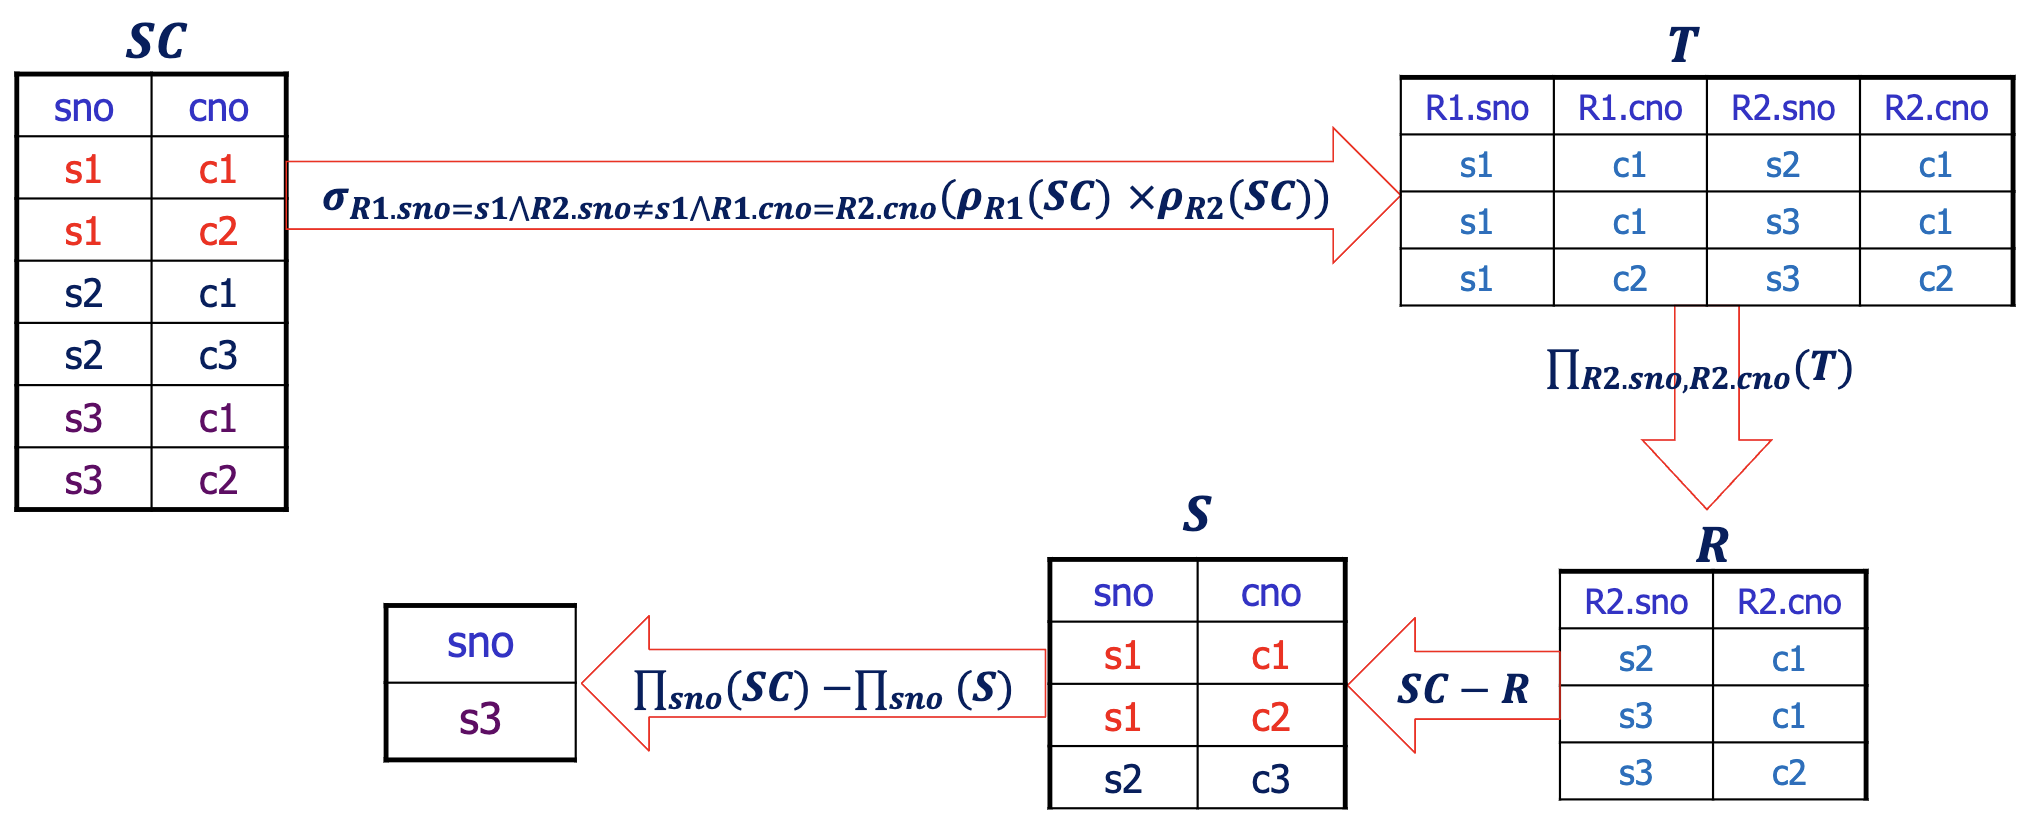
\includegraphics[width=0.8\textwidth]{./figs/2.1.png}
  \caption{示例:求其选修课程被s01号学生所修课程包含的学生号}
\end{figure}

\end{problem}  

\begin{solution}

  \begin{enumerate}
    \item 
    \[
      (\Pi_{sno}\sigma_{cno=c1}SC)\cap (\Pi_{sno}\sigma_{cno=c2}SC)
    \]
    \item 
    \[
      (\Pi_{sno}\sigma_{cno=c_1}SC)\cup(\Pi_{sno}\sigma_{cno=c_2}SC) - (\Pi_{sno}\sigma_{cno\neq c2\wedge cno\neq c1}SC)
    \]
    \item 
    \[
      (\Pi_{sno, cno}SC) \div (\Pi_{cno}\sigma_{sno=s1}SC)
    \]
    \item 反过来,先找没有被包含的
    \[
      \Pi_{sno}SC-\Pi_{sno}(SC-\Pi_{R2.sno, R2.cno}(\sigma_{R1.sno=s1\wedge R2.sno\neq s1\wedge R1.cno=R2.cno}(\rho_{R1}(SC)\times \rho_{R2}(SC))))
    \]
    \item 反过来,先求存在一样课的人
    \[
      \Pi_{sno}SC-\Pi_{R2.sno}(\sigma_{R1.sno=s1\wedge R1.cno=R2.cno}(\rho_{R1}(SC)\times \rho_{R2}(SC)))
    \]
    \item 所修课程完全相同 $\Leftrightarrow$ 所修课程被包含且包含
    \begin{align*}
      &((\Pi_{sno, cno}SC) \div (\Pi_{cno}\sigma_{sno=s1}SC))\\
      &\cap\\
      &(\Pi_{sno}SC-\Pi_{sno}(SC-\Pi_{R2.sno, R2.cno}(\sigma_{R1.sno=s1\wedge R2.sno\neq s1\wedge R1.cno=R2.cno}(\rho_{R1}(SC)\times \rho_{R2}(SC)))))
    \end{align*}
    \item 不会写

  \end{enumerate}

\end{solution}

\begin{problem}
对于关系R(A, B),用关系代数来检验A是否取值唯一。

更进一步,对于关系R(A, B, C),用关系代数来检验A是否取值唯一。

(注意,“唯一”的意思是两两不同,而不是只取同一个值,那个应该叫“单一”)  
\end{problem}

\begin{solution}

对于关系R(A, B),检查如下表达式是否为空集,如果是空集,那么说明A取值唯一,否则A取值不唯一

\[
\sigma_{R1.A=R2.A\wedge R1.B\neq R2.B}(\rho_{R1}R\times \rho_{R2}R)
\]

对于关系R(A, B, C),检查如下表达式是否为空集,如果是空集,那么说明A取值唯一,否则A取值不唯一

\[
\sigma_{R1.A=R2.A\wedge (R1.B\neq R2.B\vee R1.C\neq R2.C)}(\rho_{R1}R\times \rho_{R2}R)
\]

\end{solution}

\begin{problem}
对于选课表SC(sno, cno, grade),分别用元组关系演算和域关系演算,完成如下查询:

\begin{enumerate}
  \item 求同时选修了c1和c2课程的学生
  \item 求选修c1课程成绩比s1同学的该门课程成绩高的学生
\end{enumerate}  
  
\end{problem}

\begin{solution}

\textbf{元组关系演算:}

\begin{enumerate}
  \item 
  \[
    \{t|\exists u\exists v(u[sno]=t[sno]\wedge v[sno]=t[sno]\wedge u[cno]=c1\wedge v[cno]=c2)\}
  \]
  \item 
  \[
    \{t|\exists u(u[sno]=s1\wedge u[cno]=c1\wedge t[cno]=c1\wedge t[grade]>u[grade])\}
  \]
\end{enumerate}

\textbf{域关系演算:}

\begin{enumerate}
  \item 
  \[
    \{\left< s\right> |\exists\left< g_x\right> ,\left< g_y\right> (\left< s,c1,g_x\right> ,\left< s,c2,g_y\right> \in SC)\}
  \]
  \item 
  \[
    \{\left< s\right> |\exists\left< g\right>, \left< g1\right> (\left< s,c1,g\right> \in SC\wedge \left< s1,c1,g1\right> \in SC\wedge g> g_x)\}
  \]
\end{enumerate}

\end{solution}

\newpage
\bibliographystyle{plain}
\bibliography{ref}


\end{document}
